\vspace*{3pt}
\section{The Proposed Approach}
\label{sec:approach}

In this section, we describe the proposed approach, which utilizes
an item-based recommender system to improve test case prioritization 
techniques. 

Figure~\ref{fig:workflow} shows an overview of our proposed technique.
There are three major activities in our approach: 1) usage pattern extraction,
2) change impact analysis, and 3) test case prioritization.
The first two activities are used to produce a set of recommendations,
which is utilized to prioritize test cases. 

Before we describe these activities in detail, following is a brief overview 
of our approach and how these activities are related to each other. Note that in our approach we defined the methods as the components.

%\begin{smallitem}
\begin{itemize}
\item{Usage Pattern Extraction.} 
In this step, our goal is to calculate the frequency of usage of each component.  
The upper box in Figure~\ref{fig:workflow} shows this process.
This step contains three major parts: user session data collection,
components similarity calculation and usage rank prediction.  
The output of this step is a matrix of frequency scores for the components in method granularity. 

\item{Change Impact Analysis.} 
In this step,  we are looking for a linear model to evaluate the impact of 
change on the system. In order to measure change impact, we collect the change 
history of the applications.  We also obtain a matrix of risk scores for 
components. The lower box in Figure~\ref{fig:workflow} shows this phase.

\item{Test Case Prioritization.}
After obtaining necessary metrics of frequency and change impact scores
to produce a set of recommendations, we reorder test cases
based on these recommendations.
 
%\end{smallitem}
\end{itemize}

In the following subsections,  we will explain in detail how our recommender
system works and how we apply this technique to test case prioritization.

\begin{figure*}[!hb]
	\centering
	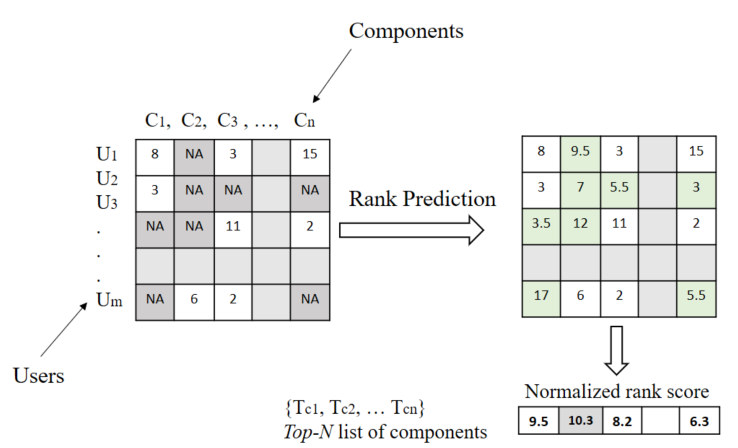
\includegraphics[width=0.75\linewidth]{./collaborative-filtring2.png}
	\vspace*{3pt}
	\caption{Collaborative Filtering Process for Identifying Most Frequent Components}
	\label{fig:collaborataivefiltering}
\end{figure*} 

\vspace*{3pt}
%\subsection{Item-Based Recommender System}
\subsection{Usage Pattern Extraction}
\label{recommender-approach}

The main focus of an item-based collaborative filtering recommender system is 
the user's rating of existing components. 
Our proposed technique uses two attributes: 
the most frequently used components and change history.

The goal of our hybrid recommender system is to suggest the highest risky 
components with the most access frequency among all other components in the applications. 
%%% why we measure frequency 
In large scale applications there are wide 
range of features and components. However, in reality 
users are not using all the functionality of the entire system. 
More often, a relatively small subset of entire system is being used by users. 
Therefore, even if a bug exist in a part of a application that 
no user ever is impacted by it, that bug has
less impact in user-perceived reliability than more frequently access components.
Our hypothesis is that by prioritizing test cases that exercise more frequently 
accessed components, we can obtain a higher rate of fault
detection of the ordered test cases. 
%%%%

To do this, we use two collected datasets: 
a list of users $U=\{u_1, u_2, ..., u_m\}$ and 
a list of our components $C =\{c_1, c_2, ..., c_n\}$. 
Each user, $u_i$, has a list of components, $c_{ui}$, that the user
has utilized in performing at least one task on $c$. 
Typically, in recommender systems, prediction is based on the numerical values of 
ratings from active users, but in our case we do not have access to such rating 
modules; instead, we consider the value of frequency access for a specific component by 
an individual active user as a rating score.

% I think I can delete this paraf %%%%%%%%%%%
There are two primary techniques for collaborative filtering algorithms:
user-based and item-based algorithms. 
In user-based collaboration filtering, we seek to find 
those users who are most similar to the current active user.
In the item-based algorithm, first we design a model of user rating, 
and then we evaluate the expected ratings of an item based on the previous 
rating of the other similar items.
%%% to here %%%%%%%%%%%


Suppose that the target user has rated a set of components,
$\{c_1, c_2,$ 
$..., c_n\}$. The item-based collaborative algorithm
computes the similarity between components by comparing the weighted average
of the target user's ratings on these similar sets of components. 
In the next phase, the algorithm selects the $k$ most similar components 
$\{c_1, c_2, ..., c_k\}$.

Further, corresponding similarities $\{s_{i1}, s_{i2}, ..., s_{ik}\}$  
between components are also estimated. After finding the 
components that are most similar, we need to predict the ratings of the
rest of the components that have been ignored or have not been used yet.
To do this, the algorithm uses a weighted average of the target user ratings
on these similar components.
Below, we describe the process of computing similarity and ranking.

Figure~\ref{fig:collaborataivefiltering} illustrates an example of
component similarity prediction.
The left-hand matrix in the picture shows how many times each component has been used
by a user, and the right-hand matrix shows the predicted similarity values.
Each number in the left matrix shows the frequency accessed by the
$i$th user on the component $C_{i}$. The numbers are in the numerical scales, and
$NA$ indicates that the user has not used that particular component yet.
To generate a list of $Top-N$ components, we need to calculate the
similarity between user usage patterns and components.
Next, we explain the process of evaluating $Top-N$ components.

In order to determine the similarity between two components $i$ and $j$, we used
Pearson-r correlation.
If $U$ is the set of users who rated components $i$ and $j$, then we compute
the correlation similarity using the following equation:

\[
{Sim (i,j) = \frac {\sum_{u\in {U}}(C_{u,i} - \bar{C_i})(C_{u,j} - \bar{C_j)}}
	{ \sqrt{\sum_{u\in {U}}({C_{u,i} - \bar{C_i}})^{2}}
		{ \sqrt{\sum_{u\in {U}}({C_{u,j} - \bar{C_j}})^{2}}}}}	
\]

where $C_{u,i}$ is the value of frequency access for user $u$ on the component $i$, and
$\bar{C_i}$ is the average value of frequency for the $i-th$ component. 

To estimate the frequency rates of ignored components, we performed
ratio prediction computation using a weighted sum method.
This method provides the ratio prediction of a specific component $i$
for user $u$ based on similar components. 

\[
{P_{u,i} = \frac {\sum_{{all\: simillar\: components , N}}(S_{i,N} * R_{u,N})}
	{\sum_{{all\: simillar\: components, N}}({S_{i,j}})}}
\]

In this equation, $R_{u,N}$ is the rating score for user $u$ and component $N$, 
and $S_{i,N}$ is the similarity score of component $i$ and $N$.
Once we calculate ratio scores for components, we can produce a matrix of components
and their frequency ranking scores;  
now we can predict the frequency access ratio for 
those components that have not been used yet.
In this step, we calculate normalized frequency scores
for components using the following equation:

\[
{F_{Ci} = \frac {{\sum}(P_{Ci})}
	{{number\: of\: users}}}
\]

where $P_{Ci}$ is the predicted rank score and $F_{Ci}$ is 
normalized rank score of component $i$. 

\vspace*{3pt}
\subsection{Change Impact Analysis}
\label{CIA-approach}

The second phase of our proposed approach is change impact analysis.
Among hundreds of attributes of code and change history metrics to evaluate
the code quality and proneness to error, we chose change history to identify
the most risky components. A previous study~\cite{raimund} indicates that
the use of change history information can be effective in detecting bugs.
The details about change impact analysis are discussed in Section~\ref{data-collection}.
After completing the feature selection phase, we designed a linear model to analyze
change impact. The output of our linear model is a matrix of components with
their change impact values, $I_{Ci}$ (the change impact score of component $i$).

\vspace*{3pt}
\subsection{Test Prioritization Using the Recommender System}
\label{test-prioritization}

After collecting the two metrics explained above (component risk scores and 
frequency ratios), we calculate the final risk score using the following equation:

\[
{ R_{Ci} = F_{Ci} * I_{Ci}}	
\]

Where $F_{Ci}$ is the frequency score of component $i$ 
and $I_{Ci}$ is the change impact score of $C_i$.  

Using $R_{Ci}$ scores, our recommender system provides a ranked list of components.
The ranked list of components contains those components of the system that are most
likely to be the cause of regression faults. 
As shown in Figure~\ref{fig:collaborataivefiltering}, the test case prioritization algorithm
reads two inputs (a recommended $Top-N$ list of components and code coverage of tests),
and reorders test cases. 

Finally, we calculate the average percentage of fault detection scores 
for the applications. 


